\section{Tcolorboxes}

\subsection{General application}
\begin{tcolorbox}[colback=red!5!white,colframe=red!50!black,title=My nice heading]
    This is a tcolorbox with a heading
\end{tcolorbox}

\begin{tcolorbox}[colback=green!5!white,colframe=green!75!black]
    Upper part of my box.
    \tcblower
    Lower part of my box.
\end{tcolorbox}

\subsection{With image}
\begin{tcolorbox}[title=Statics Problem Example, colback=white!95!black,colframe=black!70!white,colbacktitle=black!10!white, coltitle=black, fonttitle=\bfseries, coltext=black]
    \begin{center}
        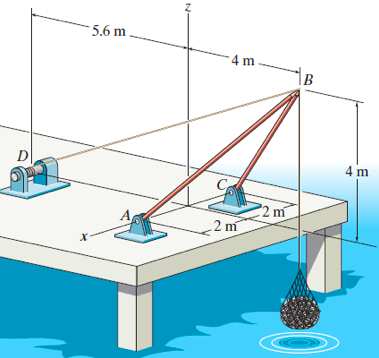
\includegraphics[width=0.5\linewidth]{photos/statics_problem.png}
    \end{center}
    The shear leg derrick is used to haul the 200-kg net of fish onto the dock. Determine the compressive force along each of the legs AB and CB and the tension in the winch cable DB. Assume the force in each leg acts along its axis.
\end{tcolorbox}